\documentclass{article}
\usepackage{amsmath}
\usepackage{amsfonts}
\usepackage{tikz}

\begin{document}

\section*{Project 1}

\subsection*{}

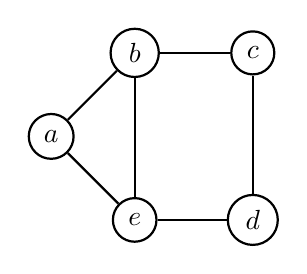
\begin{tikzpicture}[node distance={15mm}, thick, main/.style = {draw, circle}]
\node[main] (a) {$a$};
\node[main] (b) [above right of=a] {$b$};
\node[main] (e) [below right of=a] {$e$};
\node[main] (c) [right of=b] {$c$};
\node[main] (d) [right of=e] {$d$};
\draw[-] (a) -- (b);
\draw[-] (a) -- (e);
\draw[-] (d) -- (e);
\draw[-] (b) -- (c);
\draw[-] (b) -- (e);
\draw[-] (c) -- (d);
\end{tikzpicture}

\subsection*{}

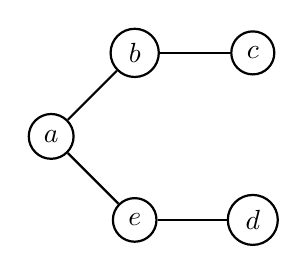
\begin{tikzpicture}[node distance={15mm}, thick, main/.style = {draw, circle}]
\node[main] (a) {$a$};
\node[main] (b) [above right of=a] {$b$};
\node[main] (e) [below right of=a] {$e$};
\node[main] (c) [right of=b] {$c$};
\node[main] (d) [right of=e] {$d$};
\draw[-] (a) -- (b);
\draw[-] (a) -- (e);
\draw[-] (d) -- (e);
\draw[-] (b) -- (c);
\end{tikzpicture}
\quad
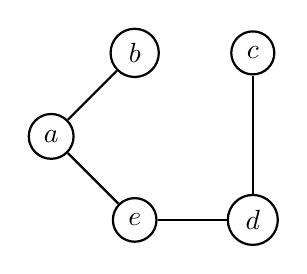
\begin{tikzpicture}[node distance={15mm}, thick, main/.style = {draw, circle}]
\node[main] (a) {$a$};
\node[main] (b) [above right of=a] {$b$};
\node[main] (e) [below right of=a] {$e$};
\node[main] (c) [right of=b] {$c$};
\node[main] (d) [right of=e] {$d$};
\draw[-] (a) -- (b);
\draw[-] (a) -- (e);
\draw[-] (d) -- (e);
\draw[-] (d) -- (c);
\end{tikzpicture}
\quad
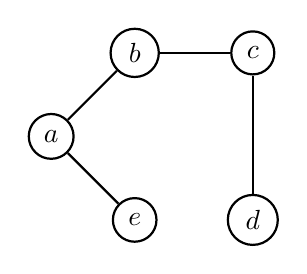
\begin{tikzpicture}[node distance={15mm}, thick, main/.style = {draw, circle}]
\node[main] (a) {$a$};
\node[main] (b) [above right of=a] {$b$};
\node[main] (e) [below right of=a] {$e$};
\node[main] (c) [right of=b] {$c$};
\node[main] (d) [right of=e] {$d$};
\draw[-] (a) -- (b);
\draw[-] (a) -- (e);
\draw[-] (b) -- (c);
\draw[-] (c) -- (d);
\end{tikzpicture}

\subsection*{}

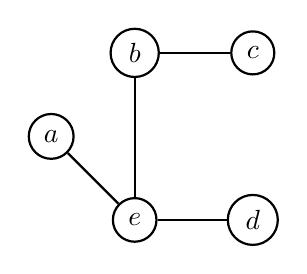
\begin{tikzpicture}[node distance={15mm}, thick, main/.style = {draw, circle}]
\node[main] (a) {$a$};
\node[main] (b) [above right of=a] {$b$};
\node[main] (e) [below right of=a] {$e$};
\node[main] (c) [right of=b] {$c$};
\node[main] (d) [right of=e] {$d$};
\draw[-] (a) -- (e);
\draw[-] (e) -- (b);
\draw[-] (b) -- (c);
\draw[-] (d) -- (e);
\end{tikzpicture}
\quad
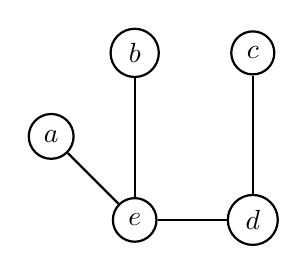
\begin{tikzpicture}[node distance={15mm}, thick, main/.style = {draw, circle}]
\node[main] (a) {$a$};
\node[main] (b) [above right of=a] {$b$};
\node[main] (e) [below right of=a] {$e$};
\node[main] (c) [right of=b] {$c$};
\node[main] (d) [right of=e] {$d$};
\draw[-] (a) -- (e);
\draw[-] (e) -- (b);
\draw[-] (c) -- (d);
\draw[-] (d) -- (e);
\end{tikzpicture}
\quad
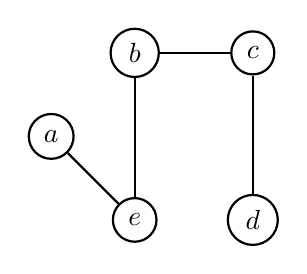
\begin{tikzpicture}[node distance={15mm}, thick, main/.style = {draw, circle}]
\node[main] (a) {$a$};
\node[main] (b) [above right of=a] {$b$};
\node[main] (e) [below right of=a] {$e$};
\node[main] (c) [right of=b] {$c$};
\node[main] (d) [right of=e] {$d$};
\draw[-] (a) -- (e);
\draw[-] (e) -- (b);
\draw[-] (b) -- (c);
\draw[-] (c) -- (d);
\end{tikzpicture}

\subsection*{}

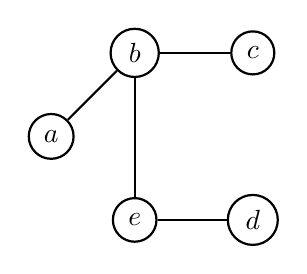
\begin{tikzpicture}[node distance={15mm}, thick, main/.style = {draw, circle}]
\node[main] (a) {$a$};
\node[main] (b) [above right of=a] {$b$};
\node[main] (e) [below right of=a] {$e$};
\node[main] (c) [right of=b] {$c$};
\node[main] (d) [right of=e] {$d$};
\draw[-] (a) -- (b);
\draw[-] (e) -- (b);
\draw[-] (b) -- (c);
\draw[-] (d) -- (e);
\end{tikzpicture}
\quad
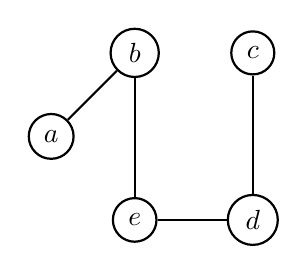
\begin{tikzpicture}[node distance={15mm}, thick, main/.style = {draw, circle}]
\node[main] (a) {$a$};
\node[main] (b) [above right of=a] {$b$};
\node[main] (e) [below right of=a] {$e$};
\node[main] (c) [right of=b] {$c$};
\node[main] (d) [right of=e] {$d$};
\draw[-] (a) -- (b);
\draw[-] (e) -- (b);
\draw[-] (c) -- (d);
\draw[-] (d) -- (e);
\end{tikzpicture}
\quad
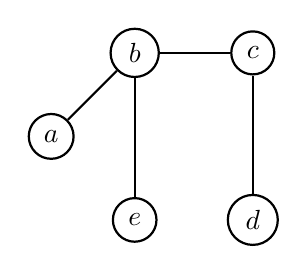
\begin{tikzpicture}[node distance={15mm}, thick, main/.style = {draw, circle}]
\node[main] (a) {$a$};
\node[main] (b) [above right of=a] {$b$};
\node[main] (e) [below right of=a] {$e$};
\node[main] (c) [right of=b] {$c$};
\node[main] (d) [right of=e] {$d$};
\draw[-] (a) -- (b);
\draw[-] (e) -- (b);
\draw[-] (b) -- (c);
\draw[-] (c) -- (d);
\end{tikzpicture}

\subsection*{}

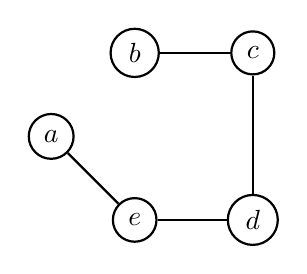
\begin{tikzpicture}[node distance={15mm}, thick, main/.style = {draw, circle}]
\node[main] (a) {$a$};
\node[main] (b) [above right of=a] {$b$};
\node[main] (e) [below right of=a] {$e$};
\node[main] (c) [right of=b] {$c$};
\node[main] (d) [right of=e] {$d$};
\draw[-] (a) -- (e);
\draw[-] (b) -- (c);
\draw[-] (c) -- (d);
\draw[-] (d) -- (e);
\end{tikzpicture}
\quad
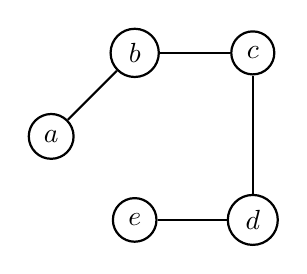
\begin{tikzpicture}[node distance={15mm}, thick, main/.style = {draw, circle}]
\node[main] (a) {$a$};
\node[main] (b) [above right of=a] {$b$};
\node[main] (e) [below right of=a] {$e$};
\node[main] (c) [right of=b] {$c$};
\node[main] (d) [right of=e] {$d$};
\draw[-] (a) -- (b);
\draw[-] (b) -- (c);
\draw[-] (c) -- (d);
\draw[-] (d) -- (e);
\end{tikzpicture}

\end{document}
